\chapter{TRACCIATO STRADALE}

Il progetto seguente consiste nello sviluppare un tronco stradale nell’ottica di una progettazione I-BIM (Infrastructure-building information modelling), ovvero un sistema di gestione e manutenzione dei processi informativi delle costruzioni infrastrutturali, in questo caso, di tipo digitale. L’obiettivo è quello di collegare con un corpo stradale i punti 7 assegnati sulla cartografia 3D di riferimento.

\begin{figure}[H]
	\centering
	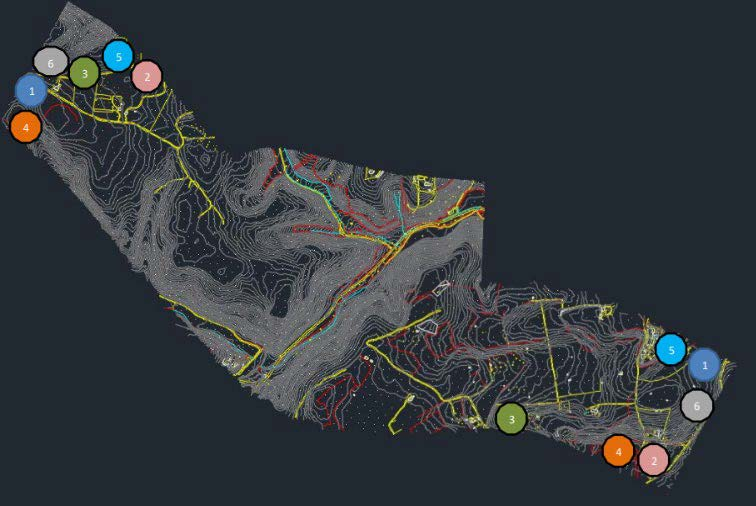
\includegraphics[width=\linewidth]{Figures/Traccia progetto}
	\captionof{figure}{Traccia progetto}
    \label{fig:Traccia progetto}
\end{figure}

Nella progettazione, tanto più è lunga la distanza tra il punto di partenza ed il punto di arrivo, tante più possibilità diverse di tracciati esistono. Per poter ottenere il tracciato definitivo si devono fare scelte opportune per limitare le spese sia in termini di difficoltà di lavorazione che in ambito economico. Inoltre, si deve tener conto anche dell’impatto ambientale dell’infrastruttura.

\section{Profilo Planimetrico}

Dopo la modellazione del terreno, per la costruzione del tracciato stradale (\ref{tracciato stradale completo}) che unisce i punti 7, si fa riferimento ad un Seed-2D, chiamato tracciato. 
Il tracciato è una raffigurazione bidimensionale dell’infrastruttura da utilizzare, ed è caratterizzato da un profilo planimetrico e da un profilo altimetrico. Per ottenere un tracciato conveniente economicamente e che non abbia un impatto ambientale troppo elevato si cerca di ottimizzare al massimo il rapporto tra terreno di scavo e terreno di riporto, facendo ciò, si cerca ridurre al massimo il volume di terreno da dover comprare o smaltire. La tecnica da utilizzare sarà quella di cercare di creare il tracciato senza tagliare troppe curve di livello, e se non se ne può fare a meno, si cercherà di ottenere un equilibrio tra discese e salite.

\begin{figure}[H]
	\centering
	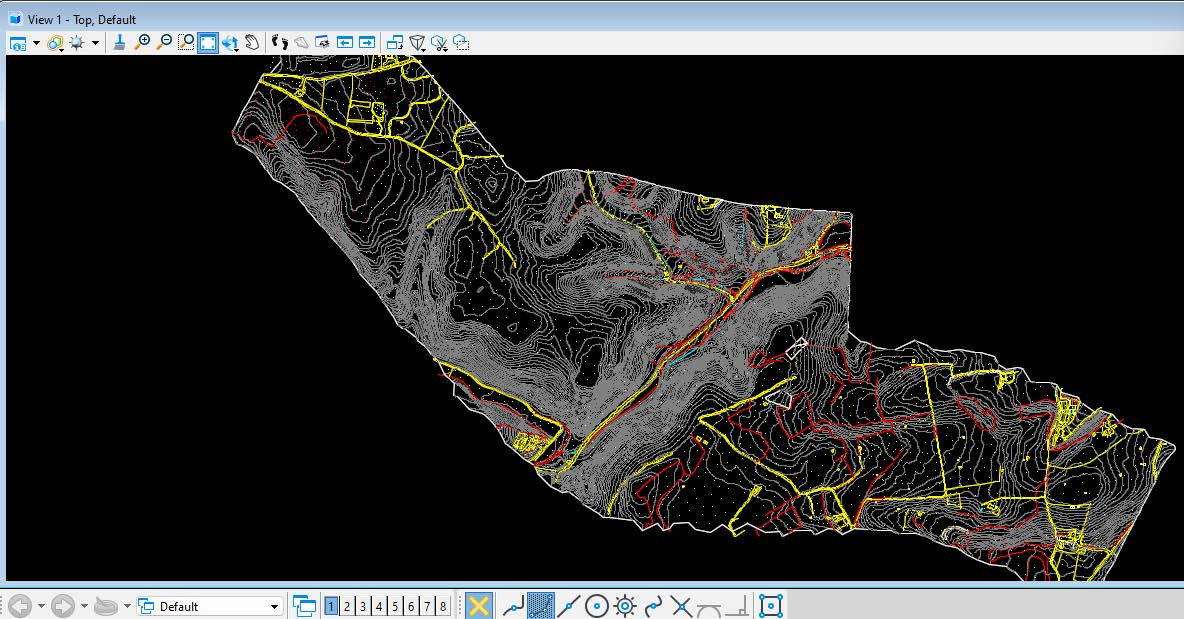
\includegraphics[width=\linewidth]{Figures/tracciato stradale completo}
	\captionof{figure}{tracciato stradale completo}
    \label{fig:tracciato stradale completo}
\end{figure}

Il profilo planimetrico è composto da una serie di rettifili, curve circolari e clotoidi, rappresentate nel programma rispettivamente in rosso, blu e giallo.
Le clotoidi possono essere di “transizione” se collegano un rettifilo e una curva circolare (cerchio arancione), di “flesso” se collegano due curve circolari di verso opposto (cerchio verde) e di “continuità” se collegano due curve con lo stesso verso di percorrenza.
La tipologia di strada che andremo a creare sarà una strada di tipo F (extraurbana). Tutti gli elementi del tracciato devono rispettare dei valori normati da:

\begin{itemize}
	\item[•] “Norme sulle caratteristiche funzionali e geometriche per la costruzione delle strade” (2001)
	\item[•] “Norme sulle caratteristiche funzionali e geometriche delle intersezioni stradali” (2006)
	\item[•] “Direttiva 2008/96/CE sulla gestione della sicurezza delle infrastrutture” (2008)
\end{itemize}

Che tengono conto del tipo di strada e del suo rispettivo intervallo di velocità di progetto.

\begin{figure}[H]
	\centering
	\includegraphics[width=\linewidth]{Figures/velocità di progetto F extraurbana}
	\captionof{figure}{velocità di progetto F extraurbana}
    \label{fig:velocità di progetto F extraurbana}
\end{figure}

La lunghezza dei rettifili deve essere tale che non si verifichino le seguenti condizioni:

\begin{itemize}
	\item[•] abbagliamento notturno da parte dei veicoli che procedono nella corsia opposta;
	\item[•] monotonia di guida dovuta ad un’eccessiva lunghezza del rettifilo;
	\item[•] impatto negativo sul paesaggio naturale;
	\item[•] superamento delle velocità consentite.
\end{itemize}

I rettifili avranno una lunghezza massima che si calcola moltiplicando la velocità massima di percorrenza per $22 (L_{max}=22*VP_{max}= 2200m)$, poi avranno una lunghezza minima tabellata.

\begin{figure}[H]
	\centering
	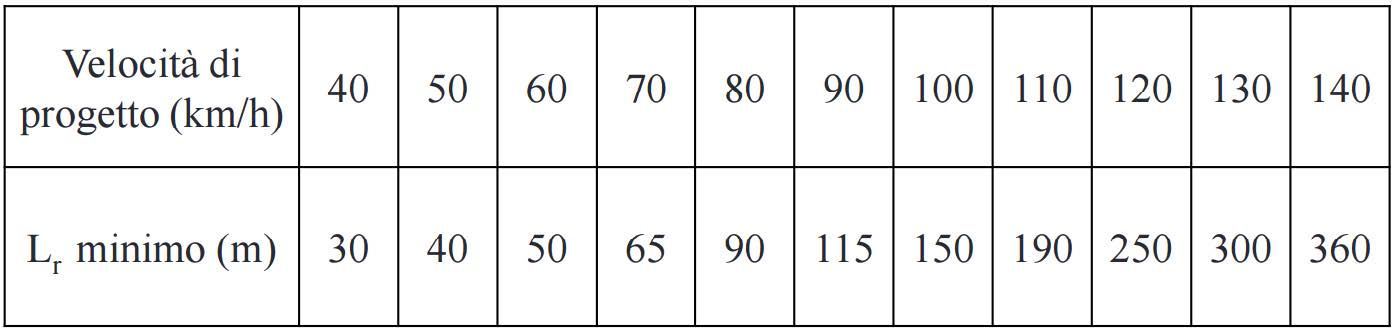
\includegraphics[width=\linewidth]{Figures/Lunghezze rettifilo minime}
	\captionof{figure}{Lunghezze rettifilo minime}
    \label{fig:Lunghezze rettifilo minime}
\end{figure}

Le curve circolari devono essere dimensionate in modo da garantire:

\begin{itemize}
	\item[•] sicurezza della circolazione, che dipende dalla stabilità e dalla visibilità;
	\item[•] comfort di marcia;
\end{itemize}

Le clotoidi invece devono necessariamente avere un fattore di scala A che rispetti i tre criteri delle norme C.N.R., ovvero il criterio dinamico che limita il contraccolpo, il criterio costruttivo che limita la pendenza relativa del ciglio esterno della carreggiata rispetto all’asse stradale e il criterio ottico che garantisce la corretta percezione ottica del tracciato.

\begin{figure}[H]
	\centering
	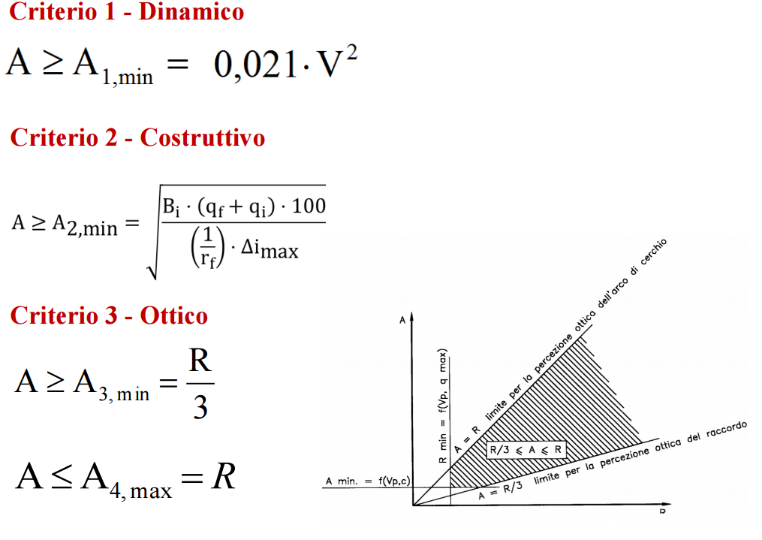
\includegraphics[width=\linewidth]{Figures/criteri di verifica}
	\captionof{figure}{criteri di verifica}
    \label{fig:criteri di verifica}
\end{figure}

Il valore più limitante è il valore dinamico, per questo motivo in fase di progetto ci si limita a verificare che sia rispettato solo il primo criterio in tutti gli elementi del tracciato.
\leavevmode
Nella pratica, per poter creare i vari elementi si utilizzerà la sezione Geometry/Horizontal utilizzando per disegnare rettifili, curve e clotoidi rispettivamente i tasti lines/line from element/spiral line from element e      ,                         arcs/arcs from element/spiral o reverse spiral arc from element.

\section{Profilo Altimetrico}

Il primo passo per creare il profilo longitudinale è quello di creare una copia del file della planimetria. Fatto ciò , bisogna indicare al programma il tipo di file DTM da cui deve prendere i dati relativi alle altezze dei punti del nostro tracciato planimetrico, per fare questo bisogna rendere attivo il DTM del terreno. Per sviluppare il profilo si userà il tasto open profile model nella sezione Geometry/Vertical, cliccando con il tasto sinistro sul tracciato, che precedentemente deve essere reso un unico elemento complesso, e poi su di una nuova vista si otterrà l’andamento altimetrico del terreno. Su di esso bisognerà costruirci le varie livellette, parabole concave e convesse.

\begin{figure}[H]
	\centering
	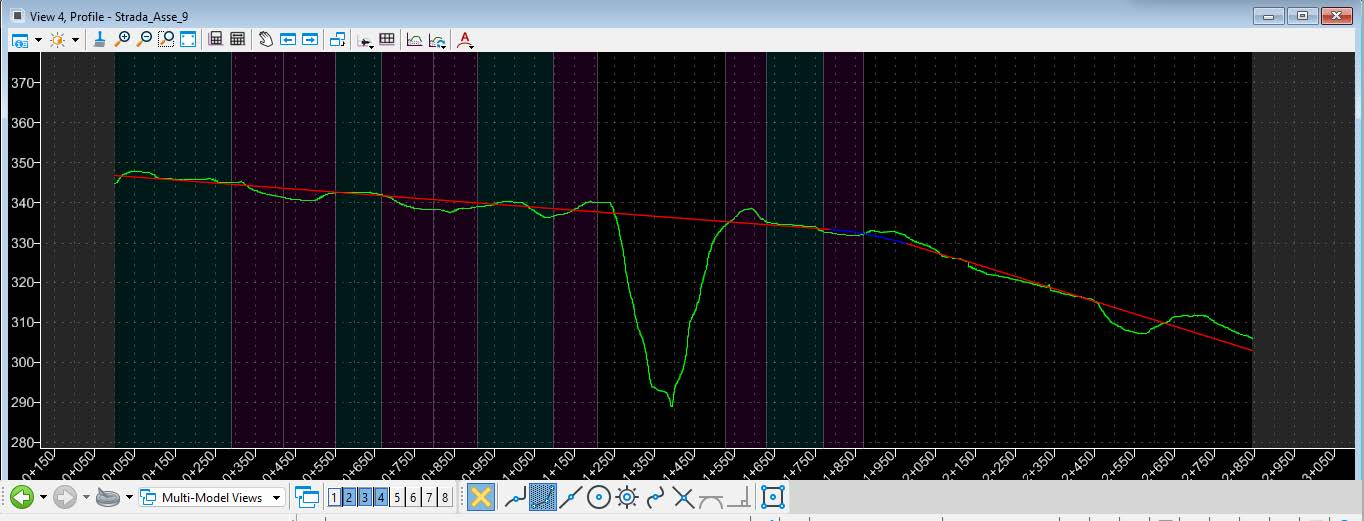
\includegraphics[width=\linewidth]{Figures/Profilo altimetrico}
	\captionof{figure}{Profilo altimetrico}
    \label{fig:Profilo altimetrico}
\end{figure}

Per disegnare il tracciato altimetrico si usa il comando (nella sezione Geometry/Vertical) Complex Geometry/ Complex Geometry By PI. Per una corretta progettazione le livellette (in rosso) vanno raccordate con raccordi parabolici concavi o convessi (in blu), in funzione del raggio o della lunghezza, purché non superino la pendenza massima del 10\%. La norma infatti stabilisce valori massimi di pendenza per evitare:

\begin{itemize}
	\item[•] in salita, rallentamenti inaccettabili (soprattutto per i mezzi pesanti), con
	consumi elevati e sforzi eccessivi per i motori;
	\item[•] in discesa, l’aumento del rischio di incidenti.
\end{itemize}

Inoltre bisogna far in modo che i vertici delle parabole siano in coincidenza della parte centrale degli elementi a raggio costante, cercare di non far capitare parabole concave sotto alla quota terreno per evitare accumuli di acqua ed infine tentare di equilibrare il quantitativo di terreno da scavare e da riportare evitando di dover fare scavi o rinterri di altezze superiori a 5 metri. Finito il tracciato altimetrico si può passare alla fase di verifiche di progetto.